\thispagestyle{toanhocvadoisongnone}
\pagestyle{toanhocvadoisong}
\everymath{\color{toanhocdoisong}}
\graphicspath{{../toanhocdoisong/pic/}}
\blfootnote{$^1$\color{toanhocdoisong}Hà Nội.}
\begingroup
\AddToShipoutPicture*{\put(0,616){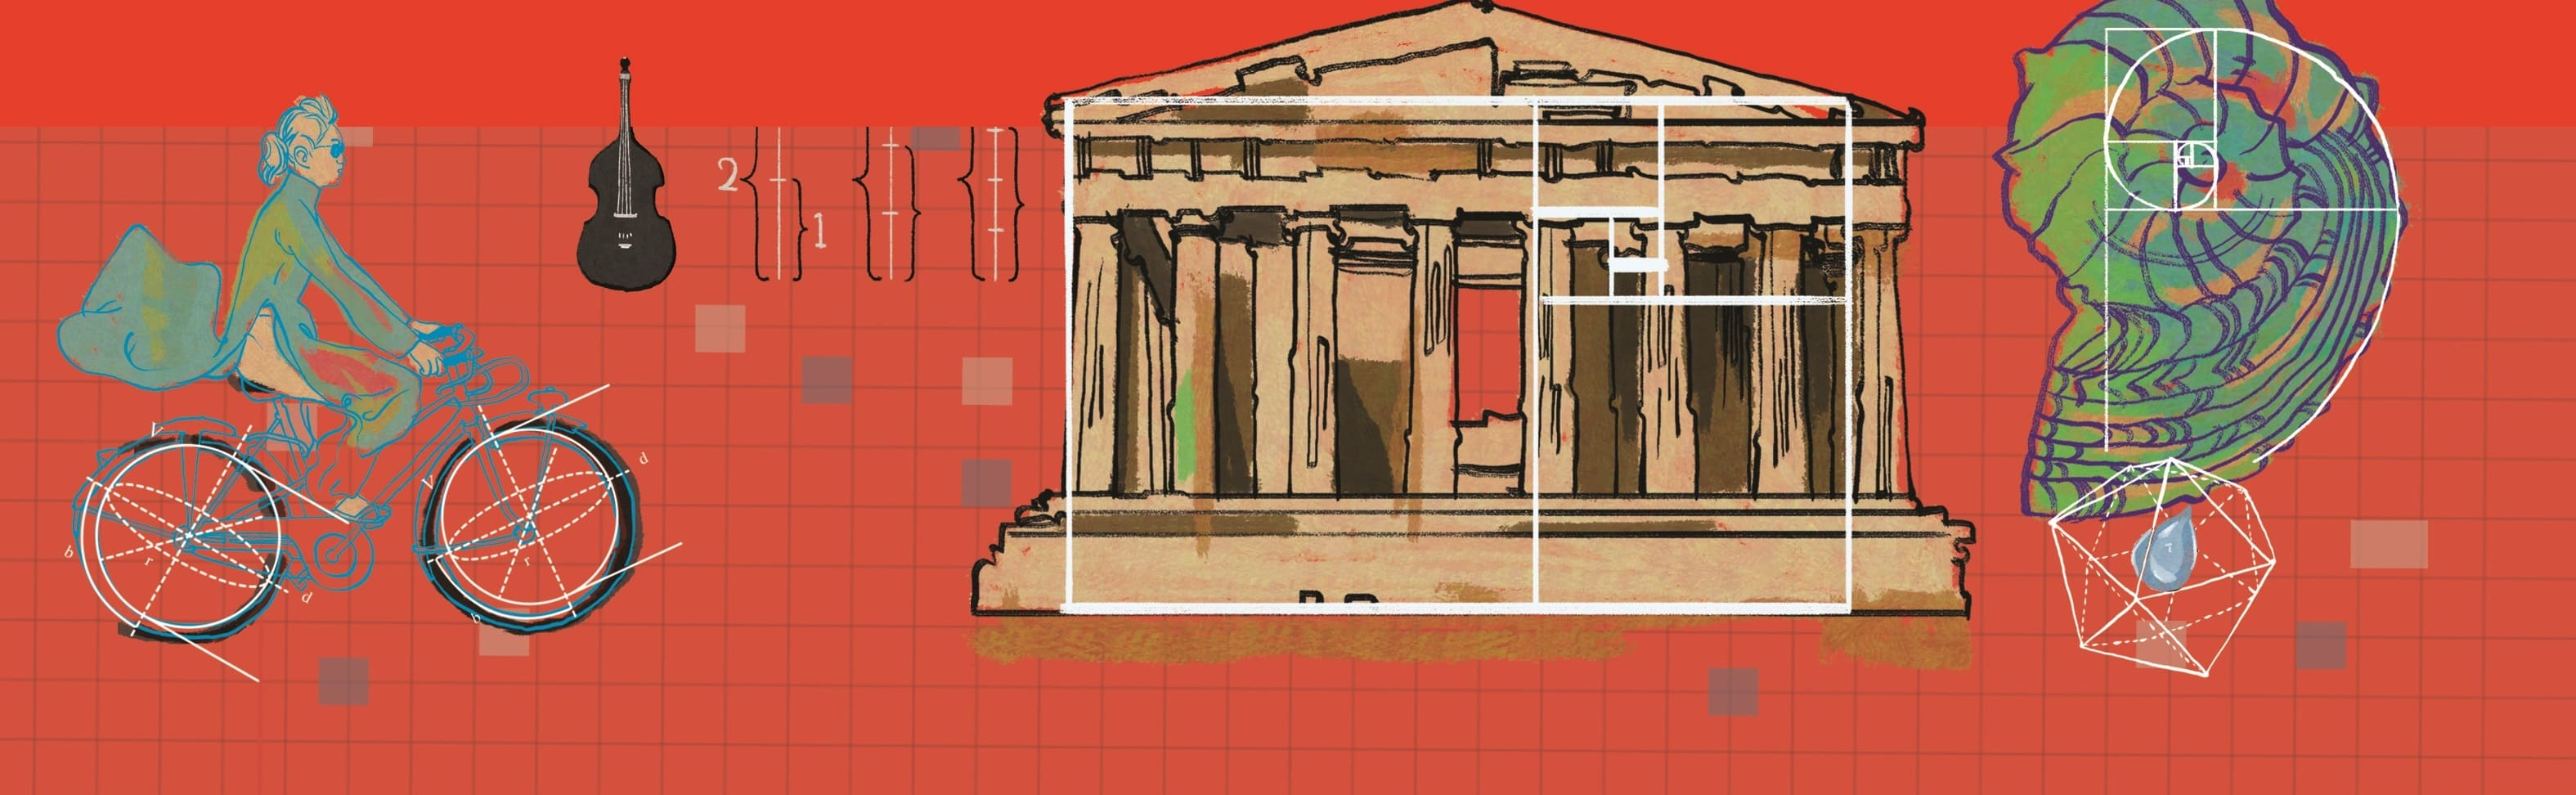
\includegraphics[width=19.3cm]{../bannertoanhocdoisong}}}
\AddToShipoutPicture*{\put(90,522){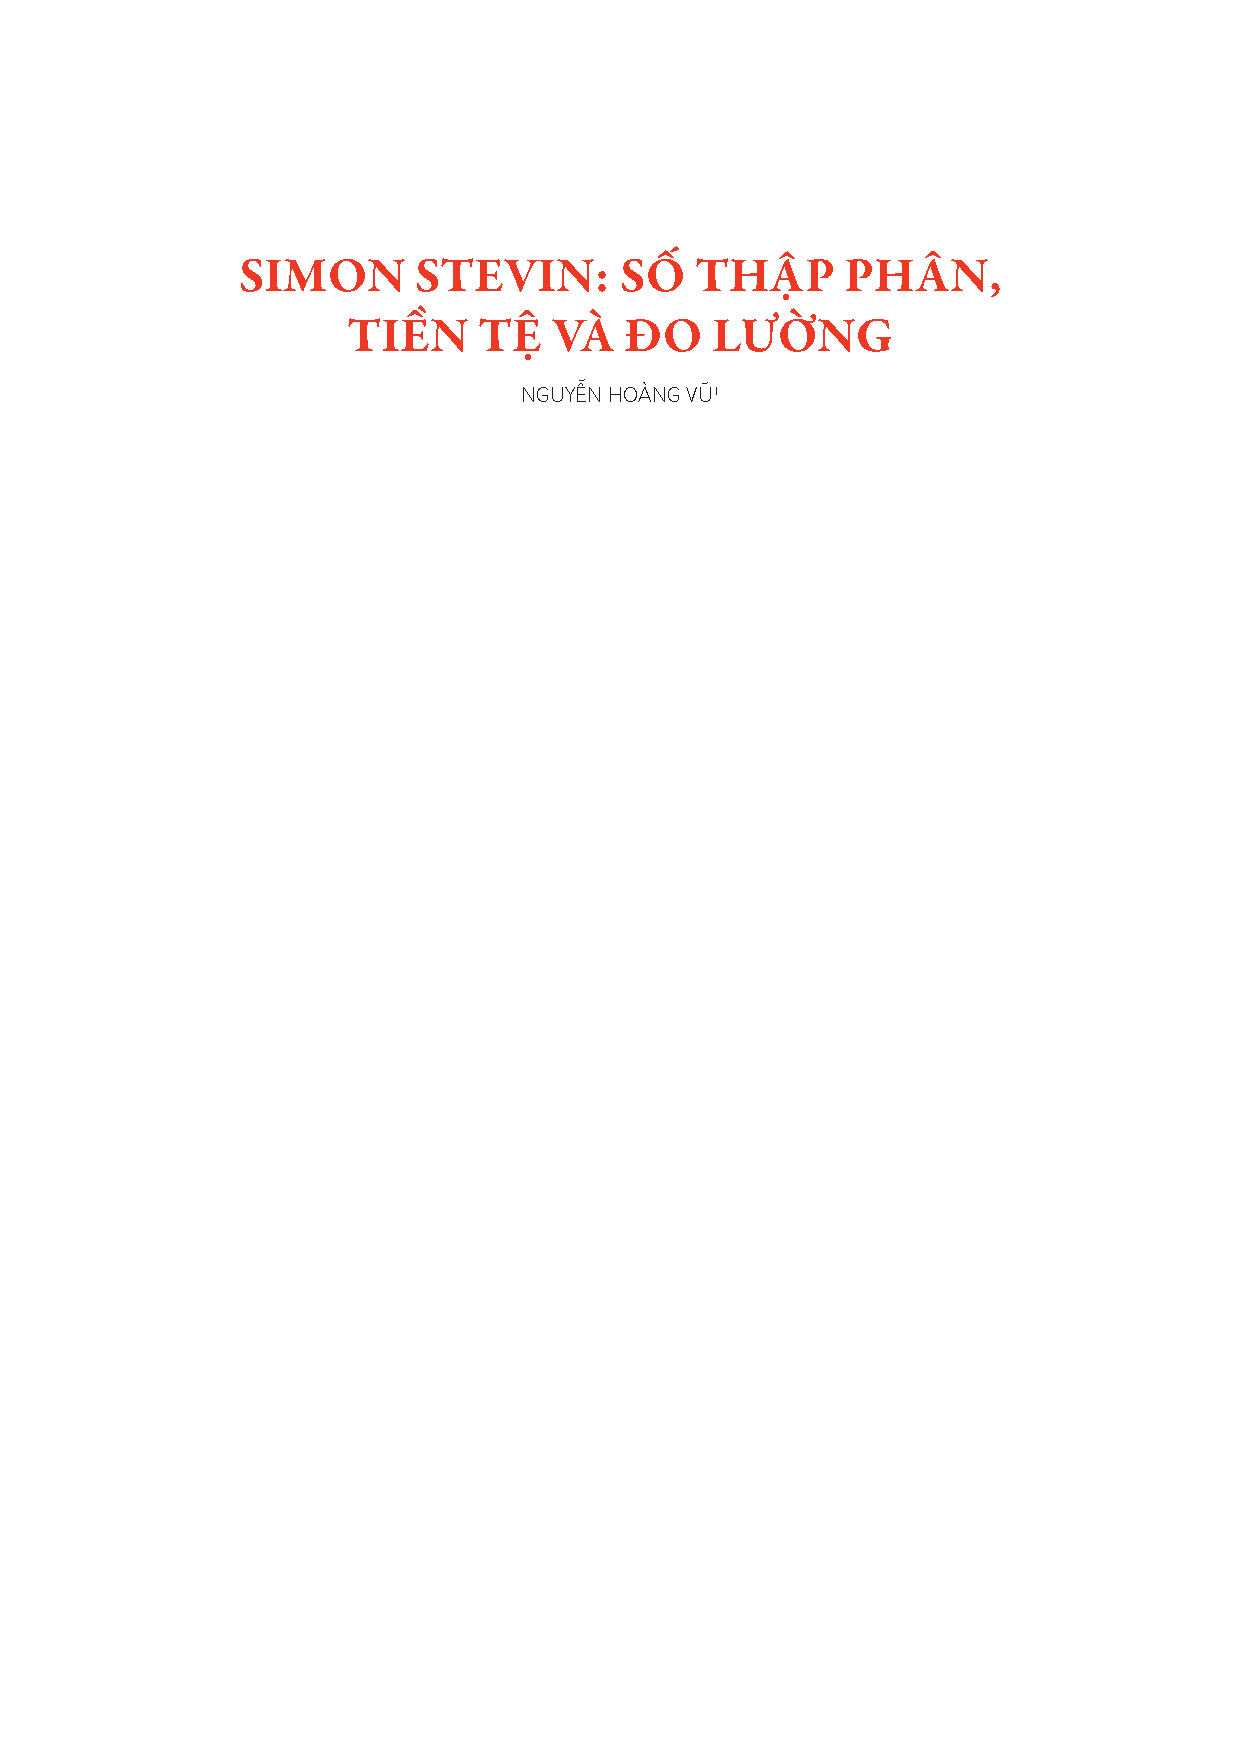
\includegraphics[scale=1]{../tieude.pdf}}}
\centering
\endgroup

\vspace*{185pt}

\begin{multicols}{2}
	Khái niệm số thập phân cũng như cách thức tính toán với chúng đã trở nên quá quen thuộc với chúng ta trong mọi mặt của đời sống. Trong bài viết này, chúng ta hãy cùng tìm hiểu việc phổ biến của số thập phân đã diễn ra như thế nào cùng một số vấn đề thực tiễn đã thúc đẩy việc sử dụng nó trong nhiều lĩnh vực khác nhau.
	\vskip 0.1cm
	$\pmb{1.}$ \textbf{\color{toanhocdoisong}Simon Stevin và De Thiende }
	\begin{figure}[H]
		\vspace*{-5pt}
		\centering
		\captionsetup{labelformat= empty, justification=centering}
		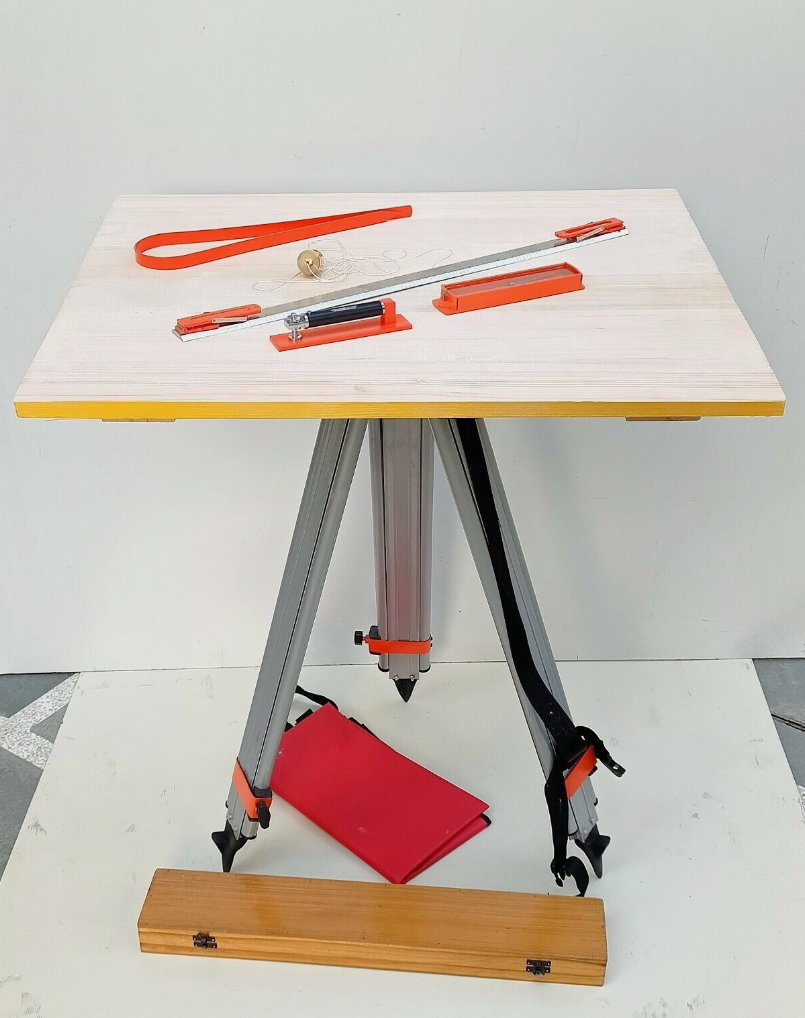
\includegraphics[width= 0.7\linewidth]{1}
		\caption{\small\textit{\color{toanhocdoisong}Simon Stevin $(1548-1620)$.}}
		\vspace*{-10pt}
	\end{figure}
	Simon Stevin sinh năm $1548$ ở Bruges (nay thuộc Bỉ). Năm $28$ tuổi, ông bắt đầu làm việc cho văn phòng thuế của thành phố rồi chuyển đến Leiden vài năm sau. Sau khi xuất bản một cuốn sách về lãi suất và một cuốn sách về hình học, năm $1583$ Stevin theo học tại đại học Leiden, vừa mới được thành lập trước đó vài năm khi Hà Lan bắt đầu phong trào đòi độc lập khỏi vương triều Habsburg của Tây Ban Nha. Trong thời gian học tại Leiden cũng như giai đoạn sau đó, Stevin viết sách về nhiều đề tài đa dang, bao gồm toán học, vật lý (đặc biệt về tĩnh học và áp suất), kinh tế, quân sự và hàng hải. Stevin là một trong những nhân vật có đóng góp quan trọng trong việc hình thành và phát triển của nước cộng hòa Hà Lan giai đoạn cuối thế kỷ $16$, đầu thế kỷ $17$.
	
	Tác phẩm \textit{De Thiende} (Nghĩa đen: Phần mười) của Stevin được xuất bản năm $1585$. Nó chỉ có $37$ trang nhưng lại có ý nghĩa rất quan trọng về mặt lịch sử bởi đây là cuốn sách đầu tiên phổ cập cách tính toán sử dụng số thập phân. Trước đó, \textit{Liber abaci} của Fibonacci sử dụng cách quy đổi hỗn số về phân số rồi chuyển ngược lại về hỗn số khi xử lý các bài toán có liên quan đến các số có phần không nguyên. Stevin đã đưa ra một cách viết số mới của mình để đơn giản hóa cách tính toán. Ví dụ, số mà ngày nay ta ký hiệu là $8,937$ được Stevin viết thành \linebreak $8$ \begin{tikzpicture}[toanhocdoisong, node font= \scriptsize]
		\draw (0,0) node[inner sep=0.5pt, draw,circle] {$0$};
	\end{tikzpicture}$9$\begin{tikzpicture}[toanhocdoisong, node font= \scriptsize]
	\draw (0,0) node[inner sep=0.5pt, draw,circle] {$1$};
\end{tikzpicture}$3$\begin{tikzpicture}[toanhocdoisong, node font= \scriptsize]
\draw (0,0) node[inner sep=0.5pt, draw,circle] {$2$};
\end{tikzpicture}$7$\begin{tikzpicture}[toanhocdoisong, node font= \scriptsize]
\draw (0,0) node[inner sep=0.5pt, draw,circle] {$3$};
\end{tikzpicture}. \begin{tikzpicture}[toanhocdoisong, node font= \scriptsize]
\draw (0,0) node[inner sep=0.5pt, draw,circle] {$0$};
\end{tikzpicture} có nghĩa rằng chữ số $8$ không được nhân với phân số nào, $9$\begin{tikzpicture}[toanhocdoisong, node font= \scriptsize]
\draw (0,0) node[inner sep=0.5pt, draw,circle] {$1$};
\end{tikzpicture} tương đương với $\dfrac{9}{10}$, $3$\begin{tikzpicture}[toanhocdoisong, node font= \scriptsize]
\draw (0,0) node[inner sep=0.5pt, draw,circle] {$2$};
\end{tikzpicture} tương đương với $\dfrac{3}{100}$ còn $7$\begin{tikzpicture}[toanhocdoisong, node font= \scriptsize]
\draw (0,0) node[inner sep=0.5pt, draw,circle] {$3$};
\end{tikzpicture} tương đương với $\dfrac{7}{1000}$. Cộng tổng của các thành phần này ta được hỗn số $8 \dfrac{937}{1000}$. Cách viết này thuận tiện ở chỗ việc cộng trừ nhân chia các số dạng này cũng tương tự như với số tự nhiên bởi bản thân các số tự nhiên viết theo kiểu Arab cũng có một đơn vị của hàng sau bằng $\dfrac{1}{10}$ một đơn vị của hàng đứng trước. Ví dụ, một phép cộng được thực hiện như dưới đây:
\begin{figure}[H]
	\vspace*{-5pt}
	\centering
	\captionsetup{labelformat= empty, justification=centering}
	\begin{tikzpicture}[toanhocdoisong]
		\draw (0,0) node {$9$};
		\draw (1,0) node {$4$};
		\draw (2,0) node {$1$};
		\draw (3,0) node {$3$};
		\draw (4,0) node {$0$};
		\draw (5,0) node {$4$};
		
		\draw[dashed]  (-0.1,0.6) -- (5.1,0.6);
		\draw (0,1) node {$8$};
		\draw (1,1) node {$7$};
		\draw (2,1) node {$5$};
		\draw (3,1) node {$7$};
		\draw (4,1) node {$8$};
		\draw (5,1) node {$2$};
		
		\draw (1,2) node {$3$};
		\draw (2,2) node {$7$};
		\draw (3,2) node {$7$};
		\draw (4,2) node {$7$};
		\draw (5,2) node {$7$};
		
		\draw (1,3) node {$2$};
		\draw (2,3) node {$7$};
		\draw (3,3) node {$8$};
		\draw (4,3) node {$4$};
		\draw (5,3) node {$7$};
		
		\draw (2,4) node[inner sep=0.5pt, draw,circle] {$0$};
		\draw (3,4) node[inner sep=0.5pt, draw,circle] {$1$};
		\draw (4,4) node[inner sep=0.5pt, draw,circle] {$2$};
		\draw (5,4) node[inner sep=0.5pt, draw,circle] {$3$};
	\end{tikzpicture}
	\vspace*{-10pt}
\end{figure}
	Cách làm này cũng không khác gì cách mà ngày nay ta cộng $27,847$ với $37,675$. Stevin cũng xét đến trường hợp có thành phần ứng với một phân số thập phân có giá trị bằng $0$, ví dụ như:
\begin{figure}[H]
	\vspace*{-5pt}
	\centering
	\captionsetup{labelformat= empty, justification=centering}
	\begin{tikzpicture}[toanhocdoisong]
		\draw (0,0) node {$1$};
		\draw (1,0) node {$3$};
		\draw (2,0) node {$6$};
		\draw (3,0) node {$3$};
		
		\draw[dashed]  (-0.1,0.6) -- (3.1,0.6);
		\draw (1,1) node {$5$};
		\draw (2,1) node {$0$};
		\draw (3,1) node {$7$};
		
		\draw (1,2) node {$8$};
		\draw (2,2) node {$5$};
		\draw (3,2) node {$6$};
		
		\draw (1,3) node[inner sep=0.5pt, draw,circle] {$0$};
		\draw (2,3) node[inner sep=0.5pt, draw,circle] {$1$};
		\draw (3,3) node[inner sep=0.5pt, draw,circle] {$2$};
	\end{tikzpicture}
	\vspace*{-10pt}
\end{figure}	
	Đồng thời, Stevin cũng trình bày cách tính căn của một số thập phân như một dạng mở rộng của việc tính căn của một số tự nhiên.
	\vskip 0.1cm
	Khác với thông lệ về sách khoa học đương thời, \textit{De Thiende} được viết bằng tiếng Hà Lan thay vì tiếng Latin. Stevin muốn cuốn sách của mình có thể được phổ biến rộng rãi nhất chứ không phải chỉ trong giới học thuật. Bản thân ông cũng tự dịch cuốn sách này sang tiếng Pháp cùng năm với bản tiếng Hà Lan. Một thời gian sau, phiên bản tiếng Đan Mạch và phiên bản tiếng Anh cũng lần lượt được xuất bản vào các năm $1602$ và $1608$.
	\vskip 0.1cm
	$\pmb{2.}$ \textbf{\color{toanhocdoisong}Tiền tệ và đo lường}
	\vskip 0.1cm
	\textit{De Thiende} không phải là một cuốn sách toán học thuần túy. Nó thuộc dòng sách về số học phục vụ tính toán trong các lĩnh vực khác nhau như tính diện tích đất đai, tính sổ sách thương nghiệp hay đo đạc phục vụ buôn bán (lương thực, rượu vang, vải vóc, ...). Stevin cho rằng việc sử dụng số thập phân sẽ giúp các công việc này được thực hiện một cách dễ dàng hơn nhiều. Tuy nhiên, điều kiện để việc này có thể được thực hiện là các đơn vị đo cũng phải được chuẩn hóa sao cho việc quy đổi các đại lượng đo được về số thập phân là dễ dàng. 
	\vskip 0.1cm
	Chẳng hạn, để đo độ dài, lúc đó người ta vẫn sử dụng các đại lượng dựa trên các đặc điểm cơ thể người: ngón cái, bàn chân, cánh \linebreak tay, ... Tuy nhiên, độ dài chuẩn của các đại lượng này luôn là vấn đề, chúng khác nhau giữa các thành phố, ngay cả cùng trong một đất nước như Hà Lan nơi Stevin sinh sống. Tình trạng tương tự cũng xảy ra với các đơn vị đo khối lượng.
	\vskip 0.1cm
	Stevin đã đưa ra ý tưởng lấy một đơn vị đo độ dài/khối lượng làm chuẩn và các đơn vị đo khác sẽ gấp $10, 100, 1000, \ldots$ lần đơn vị này hoặc bằng $1/10, 1/100, 1/1000, \ldots$ của nó. Khi đó, giá trị đo của các đại lượng thực tiễn có thể được thống nhất về cùng một chuẩn và quy đổi lẫn nhau sử dụng số thập phân. Việc tính toán với các đại lượng này cũng sẽ có thể được tiến hành dễ dàng hơn nhiều.
	\vskip 0.1cm
	Tuy rằng \textit{De Thiende} được in ấn và phổ biến ở nhiều nước châu Âu, ý tưởng đi trước thời đại này của Stevin về việc chuẩn hóa đơn vị đo sử dụng hệ thập phân chỉ được thực hiện sau đó hai thế kỷ. Ngay sau thành công của cách mạng Pháp (năm $1789$), Viện hàn lâm khoa học Pháp được yêu cầu chuẩn bị một hệ thống đo lường mới để tất cả các công dân của nước cộng hòa có thể sử dụng. Nó cần có các đơn vị chuẩn từ các đại lượng không biến thiên trong tự nhiên còn các đơn vị khác có thể được biểu diễn theo các đơn vị chuẩn này sử dụng hệ thập phân. Các nhà toán học nổi tiếng như Laplace và Lagrange cũng nằm trong hội đồng đề xuất đơn vị mới này. Năm $1799$, các đơn vị mới là mét và kilogram cũng đã ra đời, kèm theo là các đơn vị sinh ra từ các đơn vị này với các tiền tố centi, deca, \linebreak milli, ... Quá trình hoàn thiện hệ thống các đơn vị đo vẫn liên tục diễn ra với sự ra đời của hệ SI (Système International D'Unités) năm $1960$ và phiên bản chỉnh sửa năm $2019$. 
	\begin{figure}[H]
		\vspace*{-5pt}
		\centering
		\captionsetup{labelformat= empty, justification=centering}
		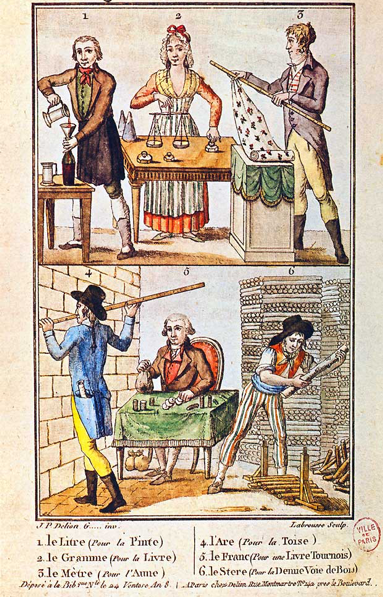
\includegraphics[width= 0.95\linewidth]{2}
		\caption{\small\textit{\color{toanhocdoisong}Hình $1$. Áp phích của chính phủ cách mạng  Pháp về việc sử dụng các đơn vị đo mới trong các lĩnh vực hàng ngày của đời sống. Việc chuyển đổi từ các đơn vị cũ sang mét và kilogram gặp nhiều khó khăn do các thói quen cũ khó biến mất ngay và cần sự thúc đấy lâu dài trong vài thập kỷ.}}
		\vspace*{-5pt}
	\end{figure}
	\vskip 0.1cm
	\PIbox{Để giảm bớt số số $0$ khi viết số thập phân, ta có thể dùng kết hợp số thập phân với các lũy thừa của $10$ khi đổi đơn vị. Ví dụ $4,1\mu m = 4,1 \times 10^{-6}m$. Cách viết này cũng giúp cho việc tính toán các đại lượng trong vật lý được thuận tiện hơn khi phần lũy thừa và phần thập phân có thể được nhân chia riêng rẽ.}
	\vskip 0.3cm
	Bên cạnh đo lường, Stevin cũng đề xuất một cải cách về tiền tệ trong \textit{De Thiende}. Trước đó, dưới thời cai trị của Tây Ban Nha, một đồng guilder vàng tương đương với $20$ đồng stuiver và mỗi đồng stuiver lại tương đương $8$ duiten hoặc $16$ penningen. Trong thời kỳ cách mạng Hà Lan, hệ thống tiền tệ lại càng hỗn loạn hơn giữa các đồng tiền đúc bằng vàng, bạc hoặc đồng. Stevin cho rằng cần có một hệ thống tiền tệ thống nhất với các đơn vị tổ chức theo hệ thập phân để thuận lợi hơn cho trao đổi và buôn bán. 
	\vskip 0.1cm
	Đề xuất về tiền tệ này của Stevin đã được thực hiện đầu tiên ở Mỹ dưới sự thúc đẩy của Thomas Jefferson. Sau khi giành độc lập khỏi đế quốc Anh vào năm $1776$, $13$ bang của nước Mỹ lúc đó vẫn dùng các loại tiền tệ khác nhau của Anh và Tây Ban Nha. Một bảng Anh (pound) bằng với $20$ shiling và một shiling bằng với $12$ xu. Tương tự, một đồng reale của Tây Ban Nha sẽ tương đương với $8$ đồng nhỏ hơn. Sự hỗn loạn về tiền tệ này gây rất nhiều khó khăn cho việc trao đổi và buôn bán trong giai đoạn mới hình thành của nước Mỹ. Thomas Jefferson, tác giả của Tuyên ngôn độc lập của Mỹ, cùng với Alexander Hamilton và Robert Morris, đã đề xuất ra hệ thống tiền tệ mới dựa trên công trình của Stevin. Năm $1785$, đồng dollar trở thành đơn vị tiền tệ của toàn nước Mỹ. Các đơn vị tiền tệ khác là disme ($\dfrac{1}{10}$ dollar tức $10$ xu) và xu (tức cent, $\dfrac{1}{100}$ dollar) được chỉ định vào năm $1792$. Các đồng tiền đúc bằng bạc đầu tiên của Mỹ là các đồng $\dfrac{1}{2}$ disme (tương đương với $\dfrac{1}{20}$ dollar). Sau này, nhiều khu vực khác nhau trên thế giới cũng dần chuyển sang hệ thống tiền tệ sử dụng hệ thập phân tương tự như nước Mỹ. Viễn cảnh về một đồng tiền sử dụng chung cho một khu vực địa lý lớn ở châu Âu của Stevin cũng thành hiện thực với sự ra đời của đồng Euro chung cho các nước EU.
	\vskip 0.3cm
	\PIbox{Khi tự dịch \textit{De Thiende} sang tiếng Pháp, Stevin chuyển tên tác phẩm là La Disme. Sau này, khi Robert Norton dịch tác phẩm này ra tiếng Anh, thuật ngữ Disme được giữ nguyên để chỉ một phần mười. Tên gọi của đồng disme tại Mỹ cũng xuất phát từ đây. Đến thế kỷ $19$, nó được viết thành dime như ta thấy trong tiếng Anh Mỹ hiện đại.
	\begin{figure}[H]
		\vspace*{-5pt}
		\centering
		\captionsetup{labelformat= empty, justification=centering}
		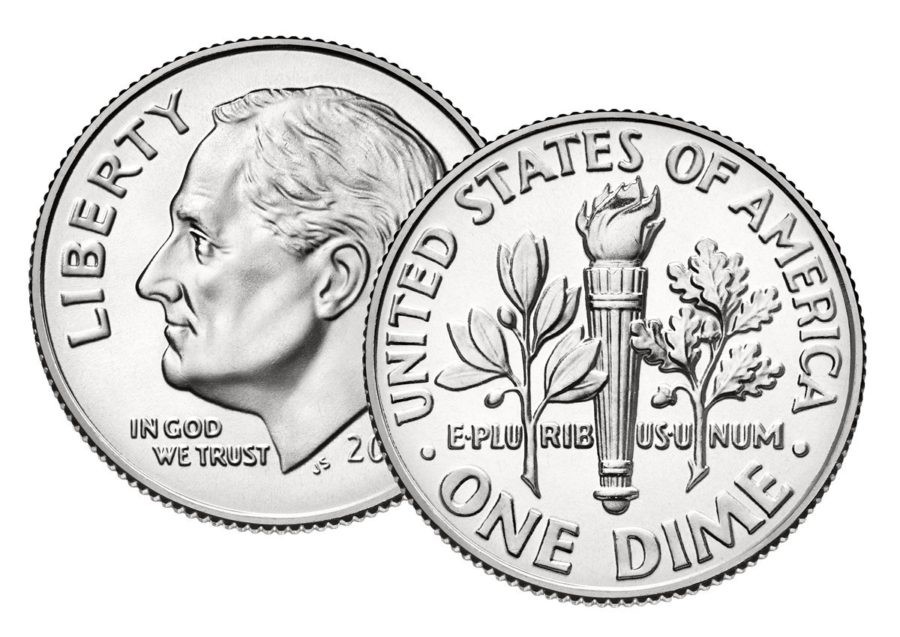
\includegraphics[height= 0.4\linewidth]{3}
		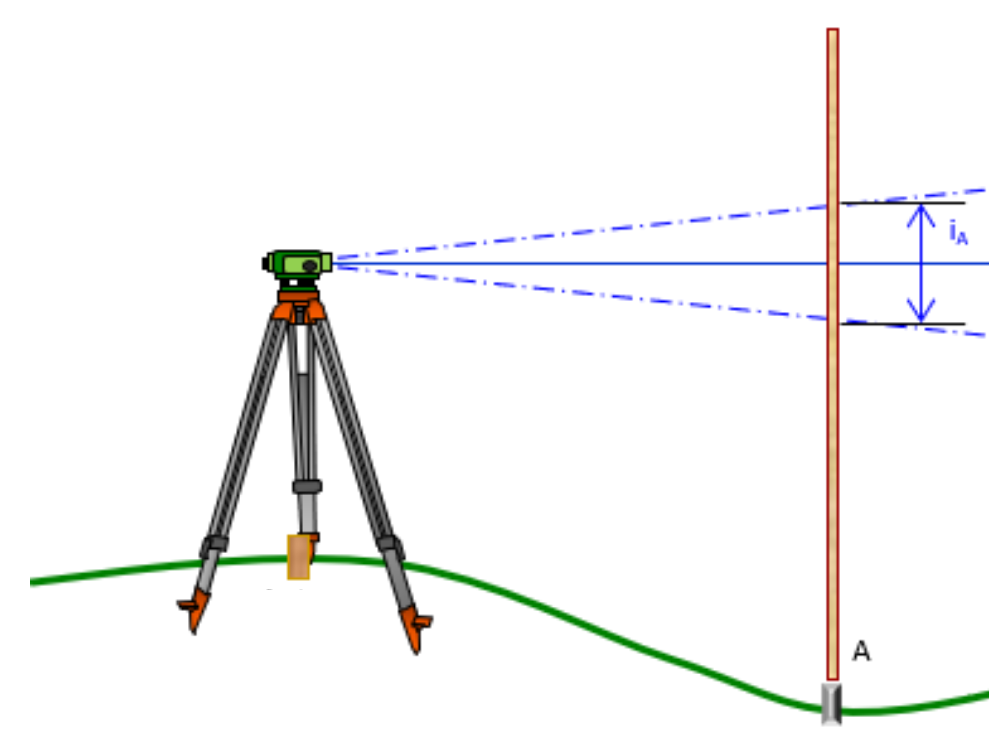
\includegraphics[height= 0.4\linewidth]{4}
		\caption{\small\textit{\color{toanhocdoisong}Trái: Đồng $10$ xu (dime) của Mỹ. Phải: Đồng $1$ xu của Mỹ với chân dung của Jefferson.}}
%		\vspace*{-10pt}
	\end{figure}
	}
	\vskip 0.3cm
	Một điều đáng chú ý là tuy Mỹ là nước đầu tiên áp dụng tiền tệ theo dạng thập phân như Stevin đề xuất, nó lại là thành trì cuối cùng trên thế giới không sử dụng rộng rãi hệ thống đo lường dạng thập phân của hệ SI. Thay vì mét và kilogram, các đơn vị từ thời đế quốc Anh như foot, yard, inch cho độ dài hay ounce và pound cho khối lượng vẫn là các đơn vị đo lường trong đời sống hàng ngày cũng như sách giáo khoa ở Mỹ. Trong thế kỷ $20$, đã có một số nỗ lực của các nhà khoa học để đưa hệ SI vào sử dụng ở Mỹ nhưng đều đã không thành công.
	\vskip 0.1cm
	\columnbreak
	$\pmb{3.}$ \textbf{\color{toanhocdoisong}Dấu chấm hay dấu phẩy}
	\vskip 0.1cm
	Khi bàn về số thập phân, ta cũng không thể không nói đến sự phức tạp của việc ký hiệu nó theo cách khác nhau trên thế giới. Đây là một vấn đề có nguồn gốc lịch sử lâu dài. Tuy cuốn sách của Stevin đã phổ cập số thập phân đến nhiều đối tượng khác nhau, cách ký hiệu của ông lại tương đối lủng củng và nhiều cách ký hiệu khác đã được đưa ra. Dấu gạch đứng ``$\mid$" được Vieta sử dụng để tách phần nguyên khỏi phần thập phân vào cuối thế kỷ $16$. Sang thế kỷ $17$, trong cuốn sách dạy tính toán sử dụng logarith của mình, Napier sử dụng cả dấu chấm lẫn dấu phẩy một cách lẫn lộn ở những phần khác nhau của quyển sách. Trước Napier, việc sử dụng dấu chấm cho số thập phân cũng xuất hiện trong một cuốn sách về thiên văn xuất bản năm $1593$ của Chrisopher Clavius. Một nghiên cứu mới gần đây (đầu năm $2024$) cho thấy việc sử dụng dấu chấm để biểu diễn số thập phân trong thiên văn học ở châu Âu như Clavius đã làm có thể có nguồn gốc từ thế kỷ $15$ trong các công trình của Giovanni Bianchini và Regiomontanus. 
	\begin{figure}[H]
		\vspace*{-5pt}
		\centering
		\captionsetup{labelformat= empty, justification=centering}
		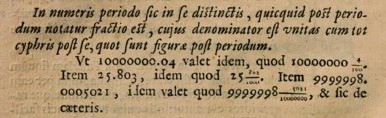
\includegraphics[width= 1\linewidth]{5}
		\caption{\small\textit{\color{toanhocdoisong}Hình $2$. Napier giải thích về số thập phân trong cuốn sách về logarith của ông. Ở trang sách này, dấu chấm được dùng để tách phần nguyên và phần thập phân.}}
		\vspace*{-10pt}
	\end{figure}
	Trong thế kỷ $17$, nhiều cách ký hiệu khác bên cạnh dấu chấm và dấu phẩy cũng xuất hiện như viết phần thập phân cao lên giống như số mũ hiện nay, gạch chân phần thập phân, sử dụng dụng ``L" để tách hai phần, sử dụng dấu chấm phẩy, ... Đến thế kỷ $18$, các cách ký hiệu mới dần ổn định. Chỉ còn lại hai trường phái chính là dấu chấm và dấu phẩy. Do Leibniz sử dụng dấu chấm để biểu thị phép nhân, phần lớn các nhà toán học châu Âu đều sử dụng dấu phẩy để ký hiệu số thập phân. Còn ở nước Anh, ký hiệu ``$\times$" vẫn được dùng phổ biến cho phép nhân và dấu chấm được sử dụng nhiều hơn cho số thập phân.
	\vskip 0.1cm
	Đến thế kỷ $19$, người Anh bắt đầu sử dụng dấu chấm trong phép nhân. Để phân biệt, dấu chấm cho số thập phân được viết giữa hai dòng kẻ còn dấu chấm cho phép nhân được viết trên dòng kẻ (ngược với cách sử dụng dấu chấm ngày nay). Trong khi đó, ở Mỹ cả hai loại dấu chấm đều được viết trên dòng kẻ. Phải đến năm $1880$, dấu chấm cho phép nhân mới được đưa lên giữa dòng như ngày nay. Đến năm $1968$, nước Anh phải đảo hai dấu chấm về giống như Mỹ để tương thích với quy định của hệ SI cho số thập phân. Cũng vào thời điểm này, tiền tệ nước Anh cũng được thập phân hóa khi đồng bảng Anh được quy tương đương với $100$ xu và các đồng $5$ xu và $10$ xu cũng bắt đầu được lưu hành. Tuy nhiên, một số tạp chí khoa học của Anh vẫn yêu cầu tác giả viết số thập phân theo cách cũ cho đến nay. Hiện tại, ngoài Anh và Mỹ, dấu chấm cho số thập phân chỉ được sử dụng ở một số nước châu Phi. Các nước còn lại trên thế giới đều sử dụng dấu phẩy còn dấu chấm thì dùng cho phép nhân. Tuy nhiên, các ngôn ngữ lập trình hiện đại đều sử dụng dấu chấm để biểu diễn số thập phân. Sự lẫn lộn về dấu chấm và dấu phẩy cũng gây khó khăn khi dữ liệu dạng số được gửi từ nước này sang nước khác. Tuy các phần mềm bảng tính như Excel đều hộ trợ việc chuyển đổi này nhưng vẫn có những vấn đề xảy ra khi việc chuyển đổi bị lỗi.
	\vskip 0.1cm
	Ở nước ta, dấu phẩy vẫn luôn được dùng cho số thập phân và đã trở thành quen thuộc. Tuy nhiên, dấu chấm cho phép nhân vẫn bị viết xuống ngang dòng kẻ thay vì giữa dòng trong rất nhiều tài liệu, bao gồm cả các bộ sách giáo khoa Toán trước kia. Nguyên nhân là do không biết hoặc tùy tiện trong việc chế bản. Trong các sách giáo khoa hiện nay, đã có bộ sách chuyển dấu chấm của phép nhân về giữa dòng nhưng cũng có bộ chưa tiến hành chuyển đổi về dạng chuẩn.
	\vskip 0.1cm
	\PIbox{Một vấn đề có liên quan là việc tách cách hàng nghìn, hàng triệu, hàng tỷ, ... ở phần nguyên. Một số nước dùng dấu chấm trong khi một số nước dùng dấu phẩy cho tránh trùng lặp với ký tự biểu diễn số thập phân. Để tránh nhầm lẫn, một số tổ chức về quy chuẩn khuyến cáo sử dụng dấu cách cho mục đích này. Ví dụ $1$ tỷ sẽ viết thành $1\, 000\, 000\, 000$.}
	\vskip 0.1cm
	$\pmb{4.}$ \textbf{\color{toanhocdoisong}Stevin và Số thập phân vô hạn}
	\vskip 0.1cm
	Trong một cuốn sách khác mang tên \textit{L'Arithmetique} (Số học), Stevin đưa ra quan điểm của mình về thế nào là một số. Ngược với các quan niệm của toán học Hy Lạp cổ đại vẫn đang thịnh hành lúc đó, Stevin cho rằng tất cả các đại lượng đo được đều có thể biểu diễn bằng số, có thể là số nguyên, số hữu tỷ hay số vô tỷ. Ông cũng cho rằng không có gì kỳ lạ với các số như $\sqrt{2}$, chúng chỉ đơn giản là những số có bình phương bằng một số khác. 
	\vskip 0.1cm
	Stevin còn đưa ra một phương pháp rất hiện đại để tìm nghiệm dưới dạng số thập phân của một đa thức. Ví dụ, với phương trình $x^3=300x+33915024$ (các hệ số được chọn để cho thấy phương pháp có thể áp dụng với đa thức dạng tổng quát), Stevin chỉ ra rằng khi $x=100$ thì về trái nhỏ hơn còn khi $x=1000$ thì vế trái lớn hơn. Do đó, sẽ có một nghiệm nằm giữa $100$ và $1000$. Sau đó ông thử các giá trị $200, 300, \ldots$ và thu hẹp khoảng nghiệm về giữa $300$ và $400$. Tiếp tục theo cách này được nghiệm là $324$. Cách làm này cũng có thể cho ra nghiệm ở dạng số thập phân vô hạn. Ví dụ $x^3=300x+33900000$ có một nghiệm nằm giữa $323$ và $324$. Ta có thể xét các nghiệm $323,1; 323,2 \ldots$ để thu hẹp khoảng nghiệm. Cứ tiếp tục và ta có thể thu được nghiệm xấp xỉ với số chữ số mong muốn ở phần thập phân. Tư tưởng của Stevin có thể nói là rất gần với những phương pháp số giải gần đúng phương trình phi tuyến hiện nay.
	\vskip 0.1cm
	Bản thân Newton cũng nói rằng số thập phân vô hạn là ý tưởng để ông phát triển khái niệm chuỗi vô hạn. Mặt khác, cách tìm nghiệm trên của Stevin cũng gần với cách Cauchy chứng minh định lý giá trị trung gian nhưng thay vì chia khoảng $[a,b]$ thành $10$ phần thì Cauchy dùng cách chia nhị phân. Stevin cũng nhận định rằng các số là liên tục chứ không phải rời rạc. Tuy nhiên, về mặt lý thuyết, phải vài trăm năm sau thì các công trình nghiên cứu của Cantor và Dedekin mới cho ta một cách xây dựng chặt chẽ về tập hợp các số thực.
	\vskip 0.1cm
	\PIbox{
	\textbf{\color{toanhocdoisong}Định lý giá trị trung gian}: Cho hàm số $f(x)$ liên tục trên khoảng $[a,b]$. Nếu $m$ là một số thỏa mãn $\min⁡\left(f(a),f(b)\right)<m< \max⁡\left(f(a),f(b)\right)$ thì tồn tại một số $c\in [a,b]$ sao cho $f(c)=m$.}
	\vskip 0.1cm
	$\pmb{5.}$ \textbf{\color{toanhocdoisong}Lời kết}
	\vskip 0.1cm
	Sự thuận tiện và đơn giản của số thập phân ngày nay làm cho chúng ta có cảm tưởng rằng nó là một phần sẵn có của toán học. Thế nhưng, đây lại là kết quả của một quá trình kéo dài với nhiều đóng góp của các nhà toán học ở các giai đoạn khác nhau. Theo một số nghiên cứu về lịch sử toán học, các cách ký hiệu số thập phân khác nhau cũng xuất hiện trong các bản thảo của al--Uqlidisi (thế kỷ $10$) và al--Kashi (đầu thế kỷ $15$) ở khu vực Trung đông. Tuy nhiên, \textit{De Thiende} của Stevin vẫn có giá trị lịch sử quan trọng nhất trong việc đưa số thập phân trở thành phổ biến bởi nó được viết không chỉ với mục đích toán học mà còn nhằm phục vụ cho đời sống, giúp cho các hoạt động thường ngày của con người diễn ra một cách dễ dàng hơn. Như đã thấy trong các số trước của Pi, Stevin còn có nhiều nghiên cứu ở các lĩnh vực khoa học khác nhau với các nghiên cứu về áp suất và trọng lực. Ông có những đóng góp không nhỏ trong việc thúc đẩy sự tiến bộ của toán học và khoa học ở châu Âu trong giai đoạn cuối của thời Phục Hưng.
	\begin{figure}[H]
		\vspace*{-5pt}
		\centering
		\captionsetup{labelformat= empty, justification=centering}
		
\includegraphics[width= 0.7\linewidth]{6}
		\caption{\small\textit{\color{toanhocdoisong}Hình $3$. Tượng Simon Stevin ở Bruges (Bỉ ngày nay), nơi ông sinh ra và lớn lên.}}
		\vspace*{-10pt}
	\end{figure}
	\vskip 0.2cm
	\PIbox{Ở Hà Lan, toán học vẫn được gọi tên bằng thuật ngữ mà Stevin đã sử dụng: wiskunde (khoa học về những điều chắc chắn).}
	\vskip 0.2cm
	\textbf{\color{toanhocdoisong}Tài liệu tham khảo}
	\vskip 0.1cm
	[$1$] Devreese, Jozef T, et al. \textit{``Magic Is No Magic" : The Wonderful World of Simon Stevin}. Southampton, Wit Press, $2009$.
	\vskip 0.1cm
	[$2$] E.J. Dijksterhuis. \textit{Simon Stevin}. Springer, $7$ Dec. $2011$.
	\vskip 0.1cm
	[$3$] Ginsburg, Jekuthiel. ``On the Early History of the Decimal Point." \textit{The American Mathematical Monthly}, vol. $35$, no. $7$, $1$ Aug. $1928$, pp. $347-347$, \url{https://doi.org/10.2307/2298362.}
	\vskip 0.1cm
	[$4$] Giunta, Carmen J. \textit{A Brief History of the Metric System}. Springer Nature, $15$ Apr. $2023$.
	\vskip 0.1cm
	[$5$] Glen Van Brummelen. ``Decimal Fractional Numeration and the Decimal Point in $15$th--Century Italy." \textit{Historia Mathematica}, $1$ Feb. $2024$, \url{https://doi.org/10.1016/j.hm.2024.01.001.}
\end{multicols}